\section{UML}


\subsection{Assoziation}

Eine \textbf{Assoziation} ist eine Beziehung zwischen mehreren Objekten (s. Abbildung~\ref{fig:association}).

\begin{figure}
    \begin{center}
        
\includegraphics[scale=0.5]{chapters/OOP/img/association}
        \caption{Beispiel für eine \textit{Assoziation} (Quelle: eigene)}
        \label{fig:association}
    \end{center}
\end{figure}

\subsection{Aggregation}


Eine \textbf{Aggregation} stellt eine Teil-Ganzes-Beziehung dar.\\
Eine offene Raute weist hier hierbei auf die Aggregat-Wurzel hin, die Linie endet bei den verschiedenen Teilen, aus denen das Aggregat besteht (s. Abbildung~\ref{fig:aggregation}).

\begin{figure}
    \begin{center}
        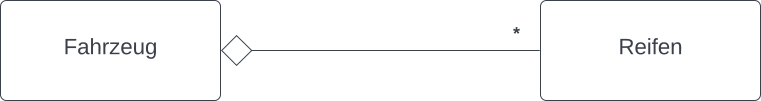
\includegraphics[scale=0.5]{chapters/OOP/img/aggregation}
        \caption{Beispiel für eine \textit{Aggregation} (Quelle: eigene)}
        \label{fig:aggregation}
    \end{center}
\end{figure}

\subsection{Komposition}

Eine \textbf{Komposition} stellt wie eine Aggregation eine Teil-Ganzes-Beziehung dar, wobei eine Komposition aus \textit{existenzabhängigen} Teilen besteht .\\
Eine gefüllte Raute weist hier hierbei auf das Ganze hin, die Linie endet bei den verschiedenen Teilen, aus denen das Kompositum besteht (s. Abbildung~\ref{fig:composition}), und die auch gelöscht werden, falls das Ganze gelöscht wird.

\begin{figure}
    \begin{center}
        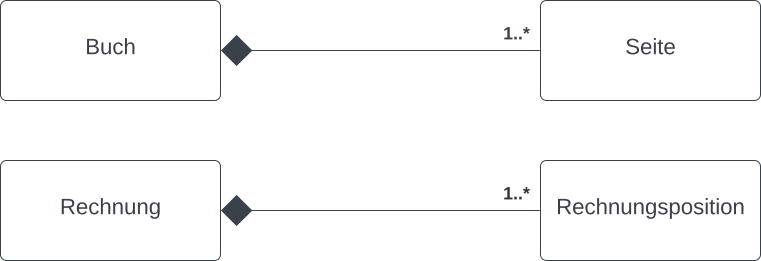
\includegraphics[scale=0.5]{chapters/OOP/img/komposition}
        \caption{Beispiel für eine \textit{Komposition} (Quelle: eigene)}
        \label{fig:composition}
    \end{center}
\end{figure}


